\documentclass[12pt,aspectratio=169,t]{beamer}
\usepackage[utf8]{inputenc}
\usepackage[T1]{fontenc}
\usepackage[french]{babel}
\usepackage{lmodern,amsmath,amssymb,booktabs,graphicx,tikz,xurl}
\usetikzlibrary{arrows.meta,positioning,calc}
\usetheme{CambridgeUS}
\setbeamertemplate{navigation symbols}{}
\setbeamertemplate{itemize items}[circle]
\setbeamertemplate{caption}[numbered]
\setbeamerfont{caption}{size=\scriptsize}
\setbeamerfont{caption name}{size=\scriptsize}
\setlength{\abovecaptionskip}{4pt}
\setlength{\belowcaptionskip}{3pt}
\AddToHook{cmd/normalsize/after}{%
  \setlength{\abovedisplayskip}{5pt plus 1pt minus 1pt}%
  \setlength{\belowdisplayskip}{5pt plus 1pt minus 1pt}%
  \setlength{\abovedisplayshortskip}{5pt plus 1pt minus 1pt}%
  \setlength{\belowdisplayshortskip}{5pt plus 1pt minus 1pt}}
\AtBeginEnvironment{figure}{%
  \setlength{\topsep}{4pt}\setlength{\partopsep}{0pt}}
\AtBeginEnvironment{table}{%
  \setlength{\topsep}{4pt}\setlength{\partopsep}{0pt}%
  \renewcommand{\arraystretch}{1.1}}
\addtobeamertemplate{itemize/enumerate body begin}{%
  \setlength{\itemsep}{4pt}\setlength{\parsep}{0pt}}{}
\setlength{\jot}{3pt}
\setbeamerfont{framesubtitle}{size=\scriptsize,shape=\upshape}
\newcommand{\question}[1]{\framesubtitle{#1}}
\newcommand{\code}[1]{\texttt{\detokenize{#1}}}
\newcommand{\python}[1]{\par\smallskip{\scriptsize\textbf{Python :} #1\par}}
\newcommand{\ii}{\mathrm{i}}
\newcommand{\dd}{\,\mathrm{d}}
\graphicspath{{../support/}}
% Valeurs issues des calculs complets en différences finies.
\newcommand{\BoundaryReflectingCost}{3,480820}
\newcommand{\BoundaryOpenCost}{0,208522}
\newcommand{\BoundaryMaterialCost}{0,416078}
\newcommand{\BoundaryOpenError}{3,916}
\newcommand{\GradientRelativeError}{\ensuremath{8{,}01\times10^{-8}}}
\newcommand{\RecommendedLevel}{0}
\newcommand{\RecommendedMaterial}{laine de verre}
\newcommand{\RecommendedBandCost}{0,627376}
\newcommand{\RecommendedCoveredNodes}{38}
\newcommand{\RecommendedRobinNodes}{128}
\newcommand{\PlanPeakFrequency}{150}
\newcommand{\PlanPeakCost}{7,141585}
\newcommand{\MonoExampleFrequency}{250}
\newcommand{\MultiBandLevelTwo}{0,942893}
\newcommand{\InitialBandLevelTwo}{1,290230}
\newcommand{\ProfileFrequency}{400}
\newcommand{\FullCostLevelZero}{0,416078}
\newcommand{\FullCostLevelOne}{0,515656}
\newcommand{\FullCostLevelTwo}{0,822255}
\newcommand{\FullCostLevelThree}{1,352007}
\newcommand{\ConfigInitialBand}{1,290230}
\newcommand{\ConfigContinuousBand}{0,476070}
\newcommand{\ConfigBinaryBand}{0,942893}
\newcommand{\ConfigMixedBand}{0,891418}
\newcommand{\ConfigFullBand}{0,822255}
\newcommand{\SelectedBandReduction}{50,95}
\newcommand{\SelectedMaximumReduction}{75,56}
\newcommand{\BestMaximumValue}{7,270847}

\title[ResoniCS -- Bruit du RER B]{ResoniCS\\Optimisation acoustique d'un mur antibruit}
\subtitle{Bruit du RER B : matériau, géométrie et placement}
\setbeamerfont{subtitle}{size=\footnotesize}
\setbeamerfont{itemize/enumerate body}{size=\small}
\author[Équipe ResoniCS]{\texorpdfstring{\footnotesize Antoine MARCHE (VT) \quad Joachim BRET (VT)\\
\footnotesize Olympia MIQUEL \quad Mathis MORET-BAILLY \quad Yann MOUSSU}{Antoine MARCHE, Joachim BRET, Olympia MIQUEL, Mathis MORET-BAILLY, Yann MOUSSU}}
\institute{CentraleSupélec}
\date{}
\hypersetup{pdfauthor={Antoine MARCHE, Joachim BRET, Olympia MIQUEL, Mathis MORET-BAILLY, Yann MOUSSU}}
\begin{document}

\begin{frame}{Présentation du projet}
\titlepage
\end{frame}

\begin{frame}{Plan}
\footnotesize
\tableofcontents
\end{frame}

\section{Cas d'usage et modèle}
\subsection{Objectif et excitation}

\begin{frame}[c]{Associer forme et matériau pour le RER B}
\question{Objectifs, état de l'art et stratégie de ResoniCS.}
\begin{itemize}
\item \textbf{Application :} diminuer le champ sonore dans un tunnel réfléchissant.
\item \textbf{Industrie :} écrans garnis de laine minérale et écrans bas près des voies. \cite{sncf,quierail}
\item \textbf{Recherche :} interfaces irrégulières et placement d'une quantité fixée d'absorbant. \cite{felix,placement}
\end{itemize}
\medskip
\centering
\textbf{Comparer le matériau, la forme et les zones garnies.}
\end{frame}

\begin{frame}[c]{Une source spectrale simplifiée du RER B}
\question{Bande de fréquences, source et paramètres physiques.}
\begin{figure}
\centering
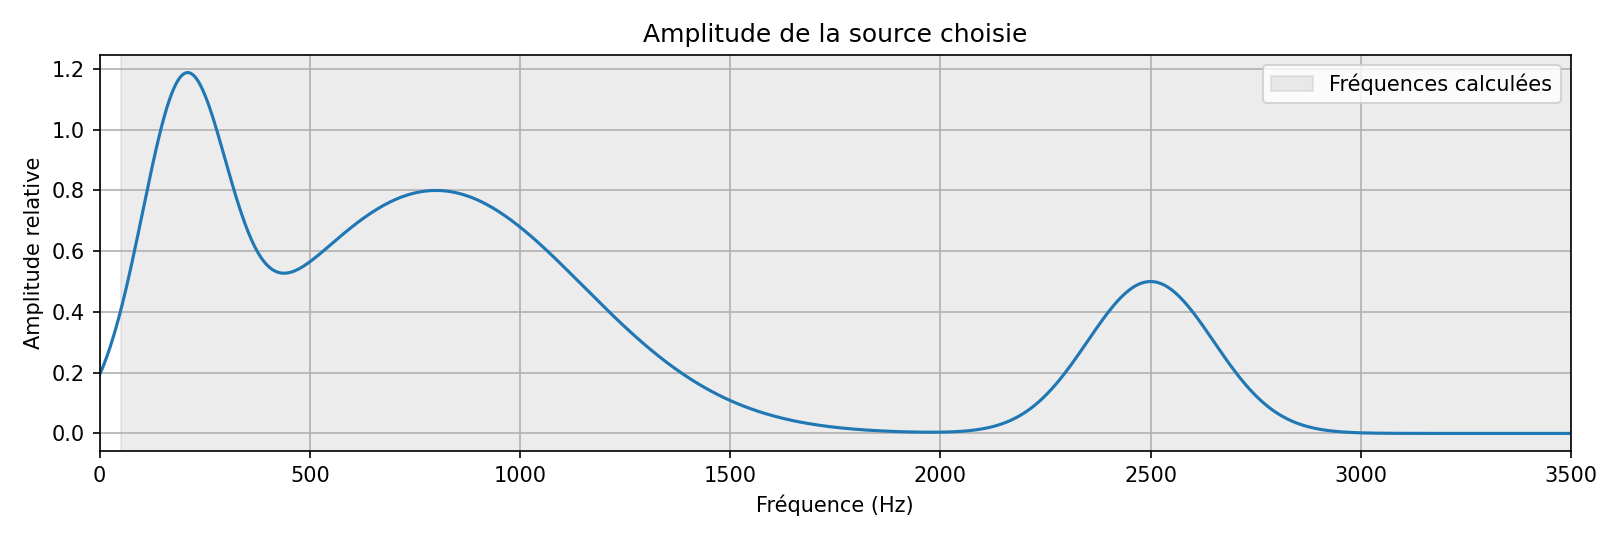
\includegraphics[width=.95\textwidth,height=.48\textheight,keepaspectratio]{fig_rer_b_spectre.png}
\caption{Amplitude de la source en fonction de la fréquence}
\end{figure}
{\small Source uniforme ; composantes à 200, 800 et 2\,500 Hz choisies pour le modèle.}
\python{\code{source_rer_b}, \code{source_constant}}
\end{frame}

\subsection{Conditions aux limites et matériaux}
\begin{frame}[c]{Propagation dans un tunnel réfléchissant}
\question{Modèle de Helmholtz et convention du coefficient de Robin.}
$\Omega$ est le domaine d'air et $u_f$ la pression complexe à la fréquence $f$.
\begin{equation*}
\begin{cases}
\Delta u_f+k_f^2u_f=0 & \text{dans }\Omega\\
u_f=g(y,\omega) & \text{sur }\Gamma_D\\
\partial_nu_f=0 & \text{sur }\Gamma_N\\
\partial_nu_f+\alpha(\omega)\chi u_f=0 & \text{sur }\Gamma_R
\end{cases}
\qquad k_f=\frac{\omega}{c}=\frac{2\pi f}{c}
\end{equation*}
\begin{itemize}
\item $n$ : normale extérieure ; $\chi$ : densité de matériau ; $\alpha$ : coefficient de paroi.
\item Convention du polycopié : $\operatorname{Re}\alpha>0$, $\operatorname{Im}\alpha<0$. \cite{cours}
\end{itemize}
\python{\code{compute_robin_condition}, \code{solve_helmholtz}}
\end{frame}

\begin{frame}[c]{Du mur plan aux contours préfractals}
\question{Géométries étudiées et échelle des irrégularités.}
\begin{figure}
\centering
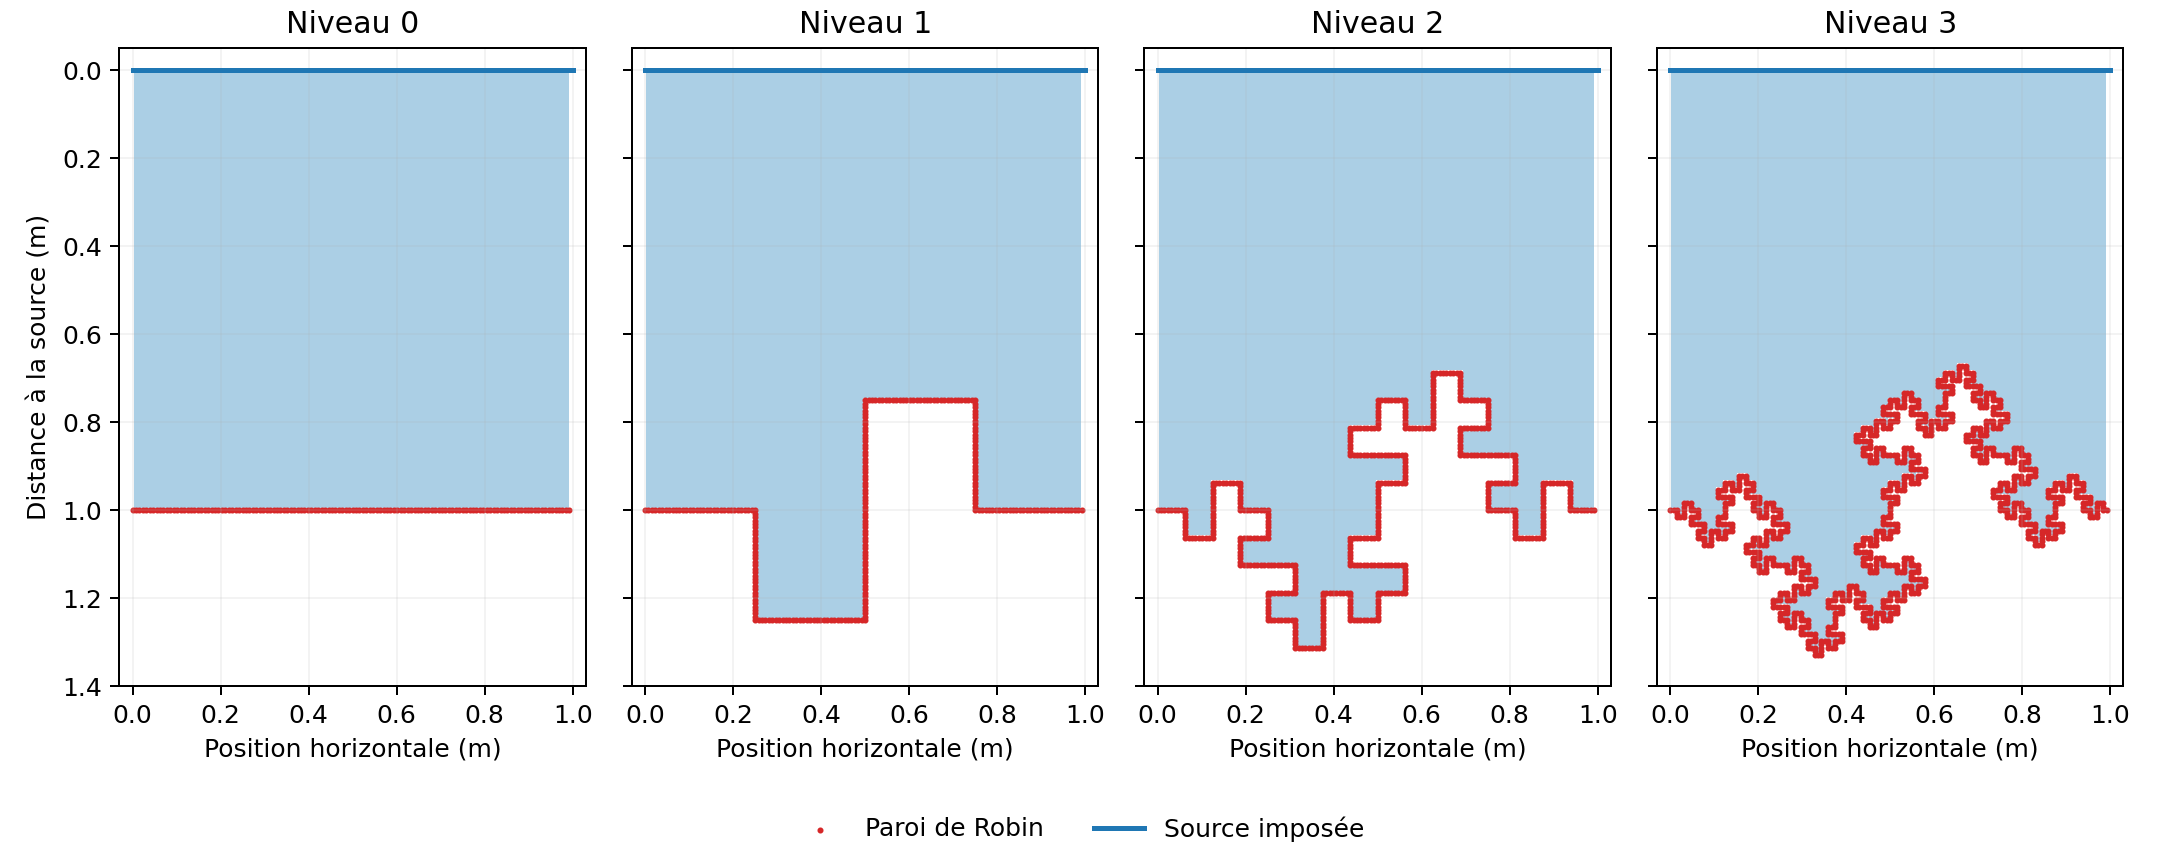
\includegraphics[width=1\textwidth,height=.50\textheight,keepaspectratio]{fig_geometries.png}
\caption{Mur plan et contours préfractals de niveaux 1 à 3}
\end{figure}
{\small Motif orthogonal répété ; le niveau modifie les reliefs et le nombre de points du mur.}
\python{\code{_set_geometry_of_domain}, \code{create_fractal_nodes}}
\end{frame}

\begin{frame}[c]{Un coefficient associé aux propriétés du matériau}
\question{Choix des matériaux poreux et identification de leur coefficient complexe.}
$\phi$ : part de pores ; $\alpha_h$ : allongement des trajets ; $\sigma$ : résistance au passage de l'air.
\begin{table}
\centering
\begin{tabular}{lrrr}
\toprule
Matériau & $\phi$ & $\alpha_h$ & $\sigma$ (Pa\,s\,m$^{-2}$)\\
\midrule
Laine de roche & 0,97 & 1,10 & 30\,000\\
Mélamine & 0,99 & 1,02 & 14\,000\\
Laine de verre & 0,99 & 1,10 & 20\,000\\
\bottomrule
\end{tabular}
\caption{Caractéristiques des trois matériaux comparés}
\end{table}
\begin{itemize}
\item On ajuste $\alpha$ pour rapprocher un modèle poreux et une condition de paroi. \cite{cours}
\item Le coefficient est recalculé à chaque pulsation, avec le même matériau.
\end{itemize}
\python{\code{MATERIAUX}, \code{materiau}, \code{compute_alpha}}
\end{frame}

\begin{frame}[c]{Variation du coefficient avec la fréquence}
\question{Comparaison des coefficients complexes des matériaux.}
\begin{figure}
\centering
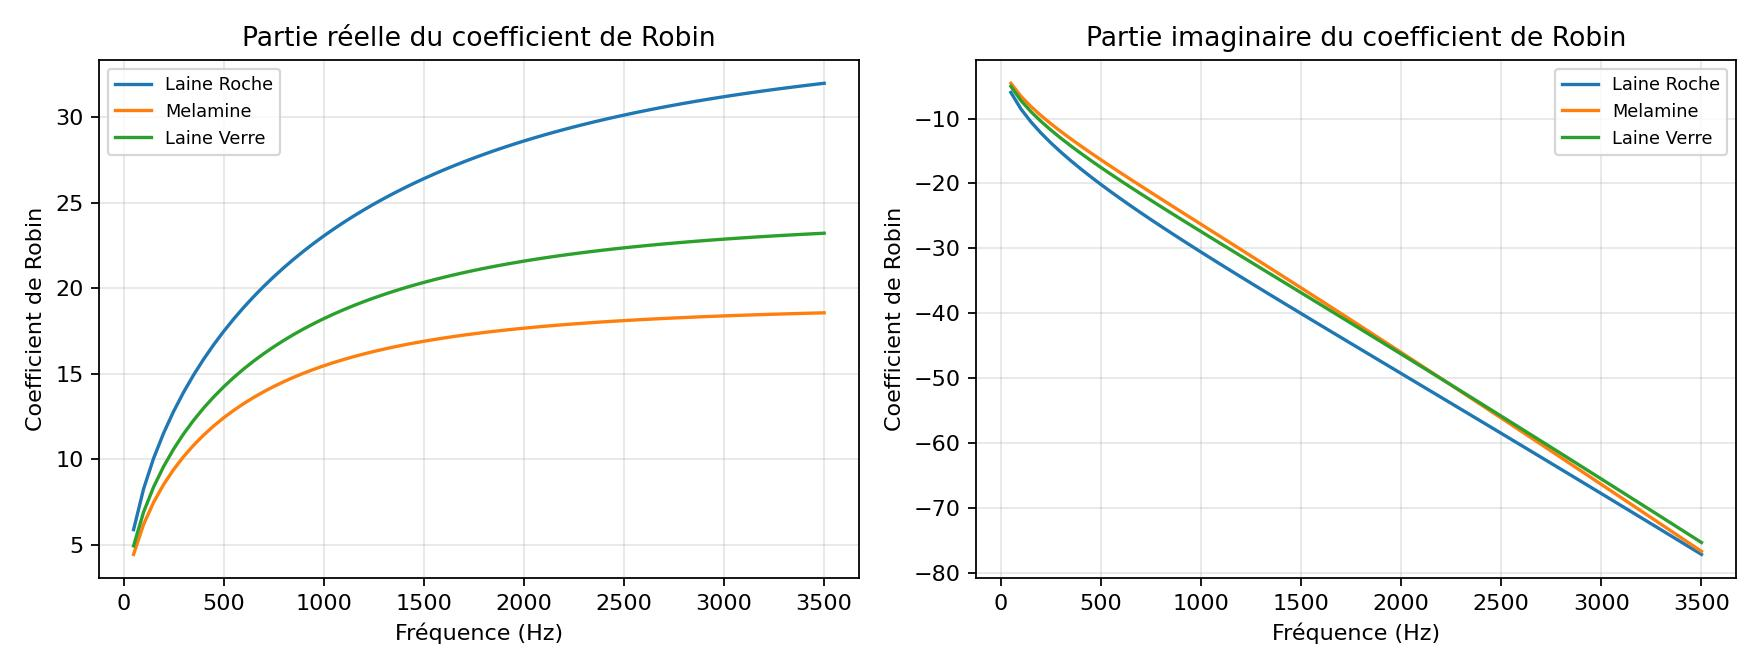
\includegraphics[width=1\textwidth,height=.50\textheight,keepaspectratio]{resultats_materiaux_validation/fig_comparaison_materiaux.jpg}
\caption{Parties réelle et imaginaire des coefficients de Robin}
\end{figure}
{\small Coefficient variable en fréquence ; comparaison des matériaux par le coût du champ.}
\python{\code{study_porous_materials}, \code{compute_material_coefficients}}
\end{frame}

\section{Méthode et vérifications}
\begin{frame}{Rappel du plan}
\footnotesize
\tableofcontents[currentsection,sectionstyle=show/shaded,subsectionstyle=show/shaded]
\end{frame}
\subsection{Critère et recherche du placement}

\begin{frame}[c]{Discrétiser les ondes et les reliefs}
\question{Méthode de résolution et résolution spatiale.}
On utilise les différences finies sur une grille de pas $h$.
\begin{equation*}
h=\frac1{128}\ \mathrm{m}
\qquad k_f=\frac{2\pi f}{343}
\qquad \lambda_f=\frac{343}{f}
\end{equation*}
\begin{itemize}
\item À 3\,500 Hz : $\lambda/h=12,544$ ; grille de $256\times128$ points.
\item Longueur des segments : $32h$, $8h$ et $2h$ aux niveaux 1, 2 et 3.
\item Niveau 3 exploratoire ; les petits reliefs et les inclusions binaires demandent un raffinement. \cite{cours}
\end{itemize}
\python{\code{_set_geometry_of_domain}, \code{create_motif_koch}, \code{FastHelmholtzSolver}}
\end{frame}

\begin{frame}[c]{Diminuer le coût à quantité de matériau fixée}
\question{Formulation du problème d'optimisation.}
Le coût mesure le module au carré de la pression dans le fluide.
\begin{equation*}
J_f(\chi)=\int_\Omega |u_f(x;\chi)|^2\dd x
\simeq h^2\sum_{j\in\Omega_h}|u_j|^2
\end{equation*}
La fraction nodale $V$ impose une quantité sur une forme donnée.
\begin{equation*}
0\leq\chi_b\leq1
\qquad \sum_{b\in\Gamma_{R,h}}\chi_b=VS
\qquad S=\#\Gamma_{R,h}
\end{equation*}
\python{\code{your_compute_objective_function}, \code{project_density}}
\end{frame}

\begin{frame}[c]{Calculer le gradient puis projeter la densité}
\question{Adjoint et descente de gradient sous contrainte.}
$U$ est le champ discret et $A(\chi)U=b(\chi)$ son système.\par
$A^*$ est la transposée conjuguée, $W$ porte les poids $h^2$ dans le fluide et $P$ désigne l'adjoint.
\begin{equation*}
A(\chi)^*P=2WU
\qquad
D J[\delta\chi]=\operatorname{Re}\!\left(P^*(\delta b-\delta A\,U)\right)
\end{equation*}
On projette la proposition dans l'ensemble admissible, puis on accepte le pas si son coût diminue.
\begin{equation*}
\chi^{n+1}=\Pi_{[0,1],\,\sum\chi=VS}\!\left(\chi^n-\mu_n\nabla J(\chi^n)\right)
\end{equation*}
\begin{itemize}
\item Le tri final fournit une répartition binaire, dont on recalcule le coût.
\end{itemize}
\python{\code{compute_adjoint}, \code{compute_gradient}, \code{binarize_chi}}
\end{frame}

\subsection{Cas de contrôle}
\begin{frame}[c]{Comparer une paroi ouverte et une paroi réfléchissante}
\question{Énergie avec une frontière ouverte et comparaison au cas réfléchissant.}
\begin{figure}
\centering
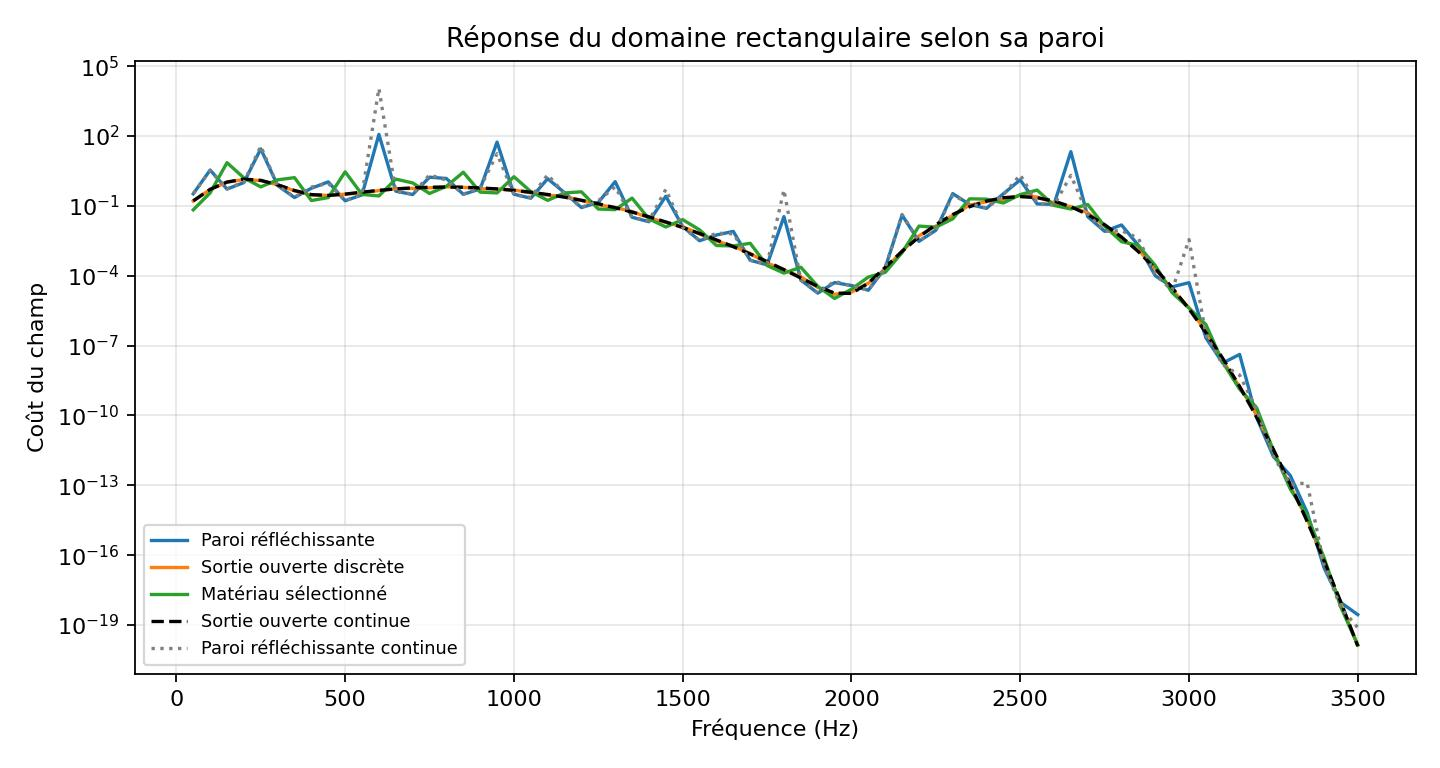
\includegraphics[width=.98\textwidth,height=.50\textheight,keepaspectratio]{resultats_materiaux_validation/fig_sommerfeld_vs_reflexif.jpg}
\caption{Coûts du champ pour trois conditions de paroi}
\end{figure}
{\small Sortie ouverte : $\partial_nu-\ii k_fu=0$ ; comparaison aux solutions continues.}
\python{\code{study_sommerfeld_open_air_vs_reflexive}}
\end{frame}

\begin{frame}[c]{Observer l'effet de la forme à aire constante}
\question{Coût du modèle continu selon la profondeur du rectangle.}
\begin{figure}
\centering
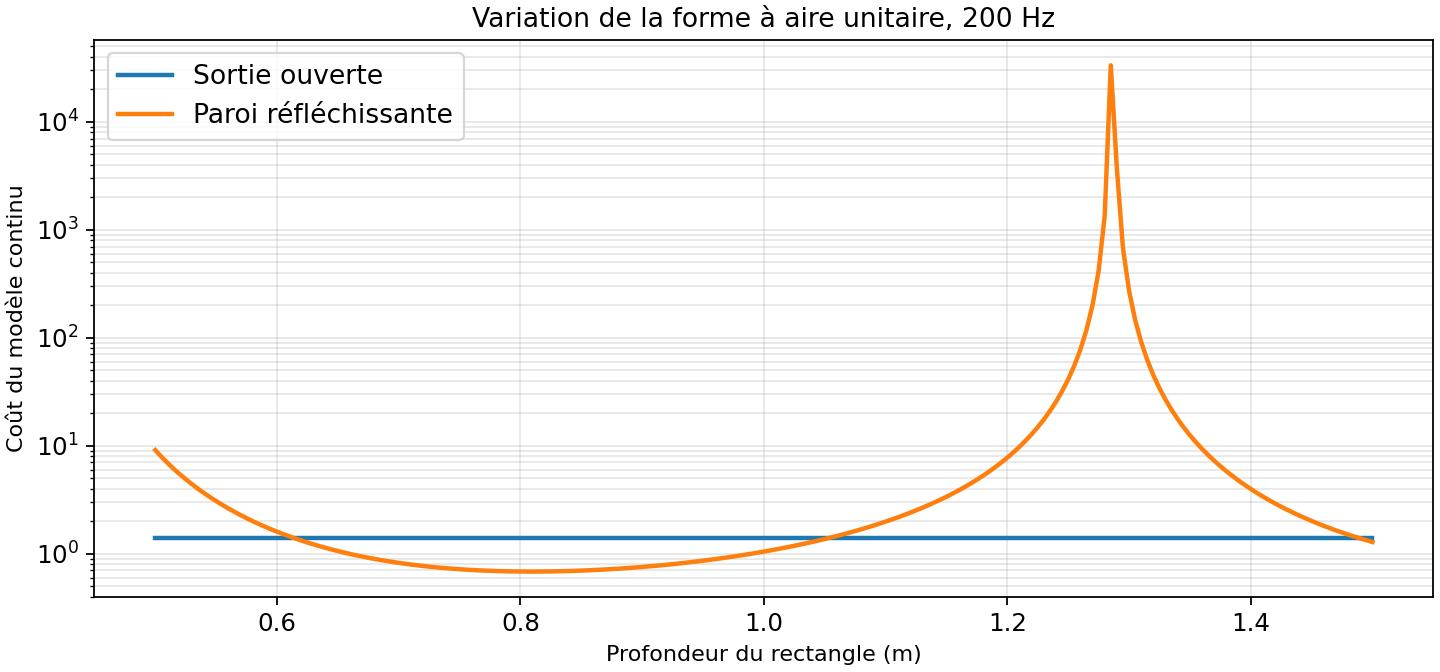
\includegraphics[width=.98\textwidth,height=.48\textheight,keepaspectratio]{resultats_materiaux_validation/fig_cout_profondeur_rectangle.jpg}
\caption{Coût en fonction de la profondeur à 200 Hz}
\end{figure}
{\small Largeur $w=A_\Omega/d$, avec $A_\Omega=1\,\mathrm{m^2}$ : coût ouvert constant.}
\python{\code{study_boundary_depth_dependence}}
\end{frame}

\begin{frame}[c]{Vérifier la dérivée calculée par l'adjoint}
\question{Contrôle numérique du gradient par perturbation de la densité.}
\begin{figure}
\centering
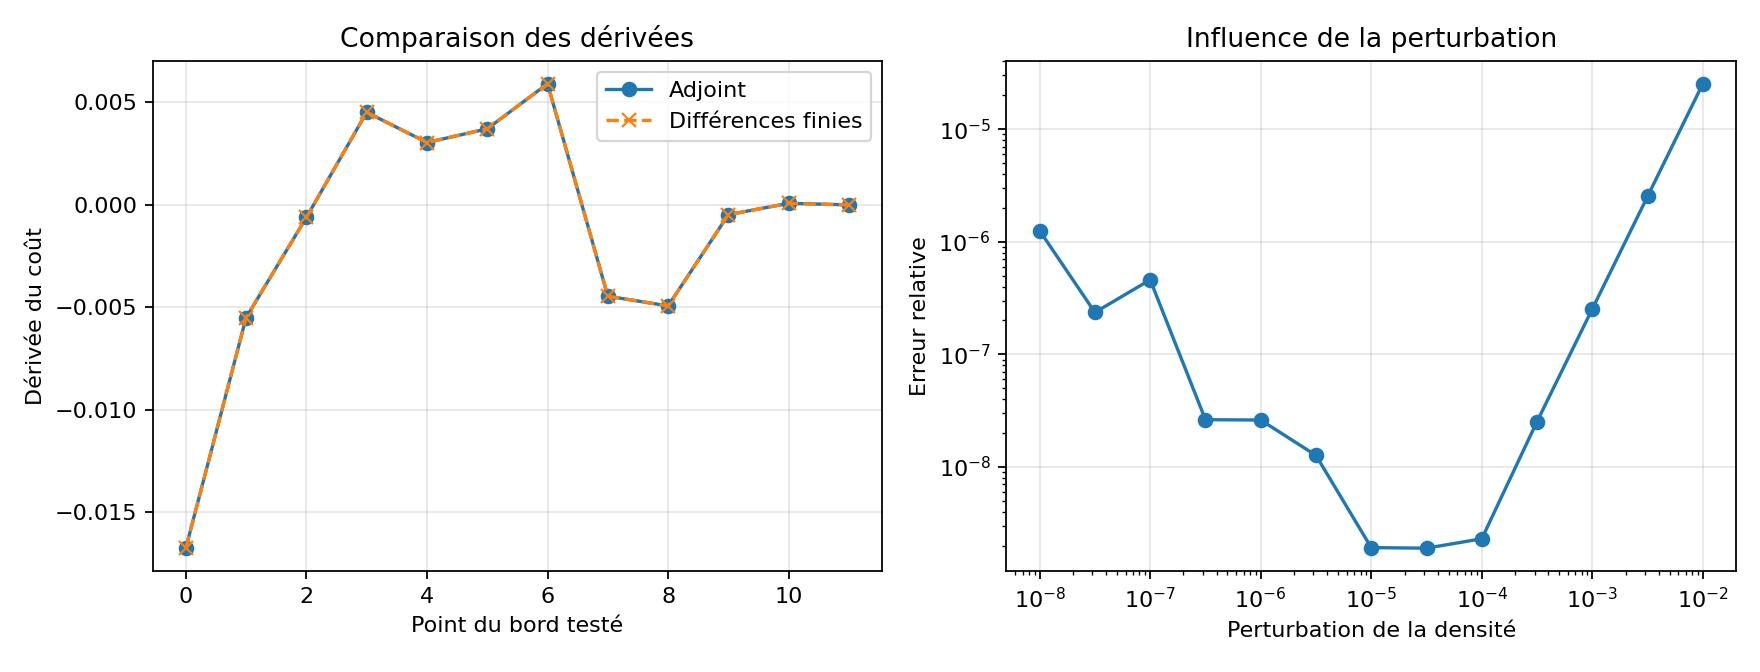
\includegraphics[width=1\textwidth,height=.50\textheight,keepaspectratio]{resultats_materiaux_validation/fig_validation_gradient_adjoint.jpg}
\caption{Gradient adjoint et différences finies}
\end{figure}
{\small Douze points testés par perturbation ; erreur relative : $\GradientRelativeError$.}
\python{\code{validate_adjoint_gradient}}
\end{frame}

\section{Spectres et placement à une fréquence}
\begin{frame}{Rappel du plan}
\footnotesize
\tableofcontents[currentsection,sectionstyle=show/shaded,subsectionstyle=show/shaded]
\end{frame}
\subsection{Formes et maxima locaux}

\begin{frame}[c]{Repérer les fréquences problématiques du mur plan}
\question{Spectre d'un mur plan entièrement garni et maxima locaux.}
\begin{figure}
\centering
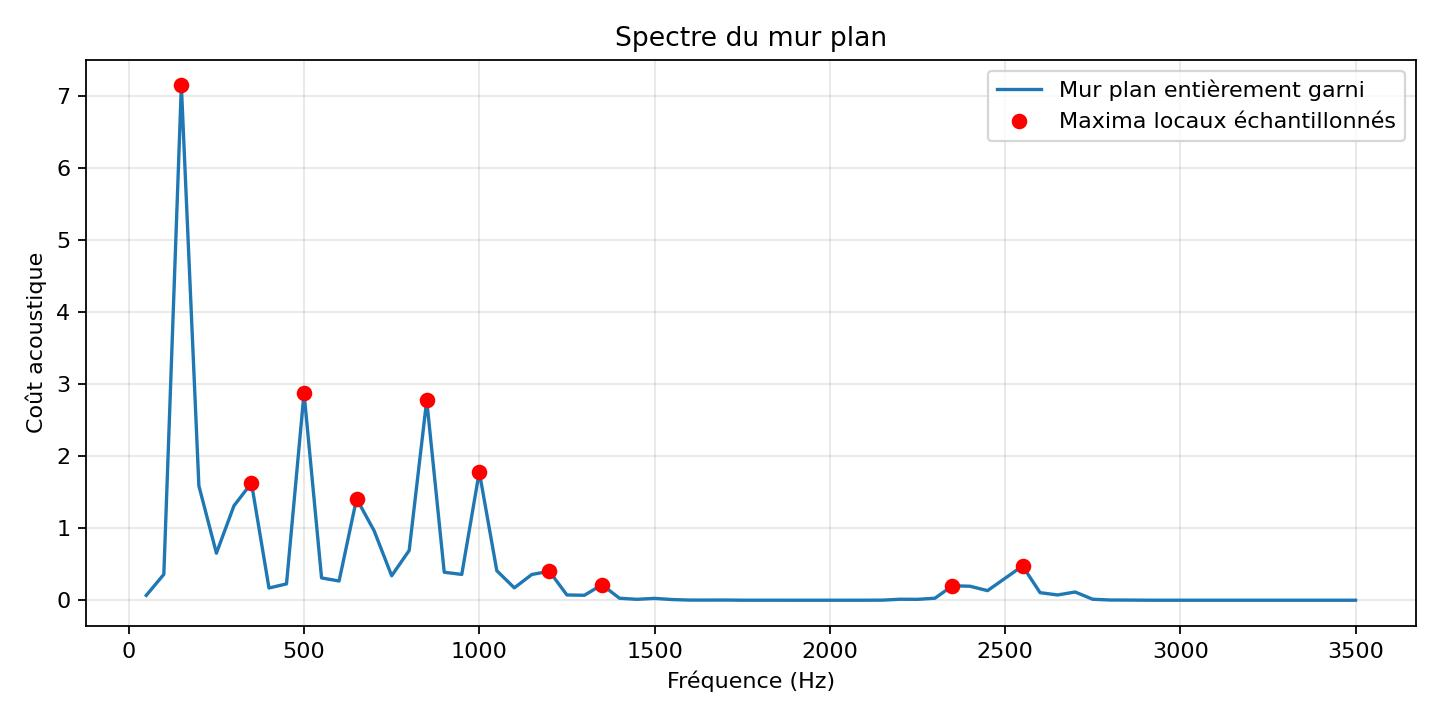
\includegraphics[width=1\textwidth,height=.50\textheight,keepaspectratio]{resultats_monofrequence/fig_mur_plan_absorbant_maxima.jpg}
\caption{Coût du mur plan en fonction de la fréquence}
\end{figure}
{\small 70 fréquences espacées de 50 Hz ; maxima repérés sur la grille échantillonnée.}
\python{\code{evaluate_spectrum}, \code{find_local_maxima}}
\end{frame}

\begin{frame}[c]{Comparer les formes de murs entièrement garnis}
\question{Spectres des géométries planes et préfractales.}
\begin{figure}
\centering
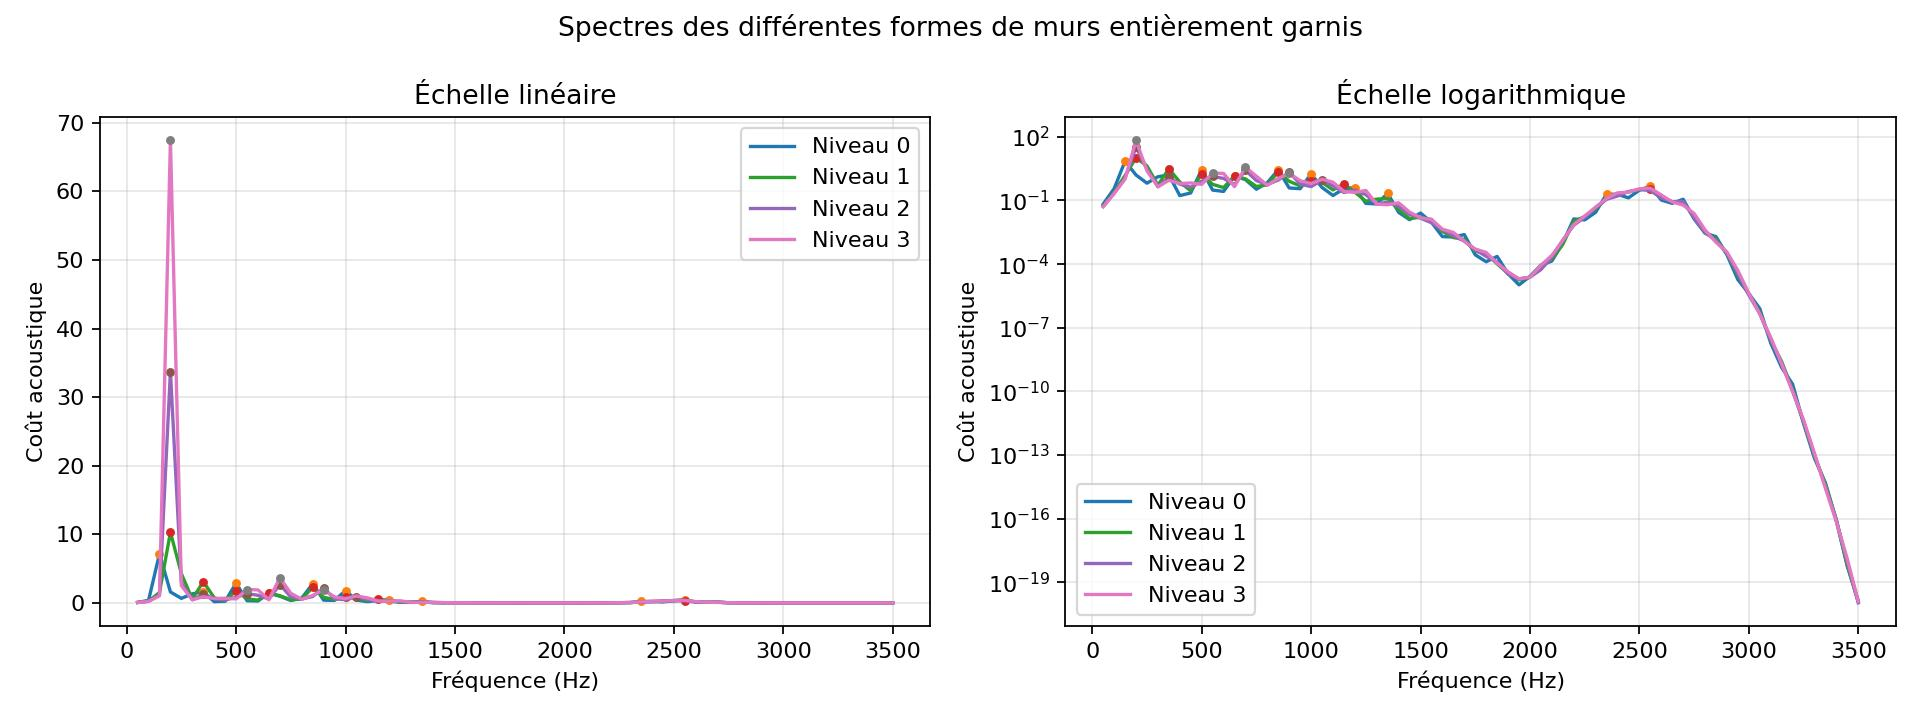
\includegraphics[width=1\textwidth,height=.50\textheight,keepaspectratio]{resultats_monofrequence/fig_comparaison_formes_fractales.jpg}
\caption{Spectres des murs de niveaux 0 à 3}
\end{figure}
{\small Même source et même matériau ; quantité totale garnie variable avec le contour.}
\python{\code{study_spectra_and_single_frequency_placement}}
\end{frame}

\subsection{Placement à quantité fixée}
\begin{frame}[c]{Comparer un mur partiellement et entièrement garni}
\question{Répartition initiale et référence entièrement garnie.}
\begin{figure}
\centering
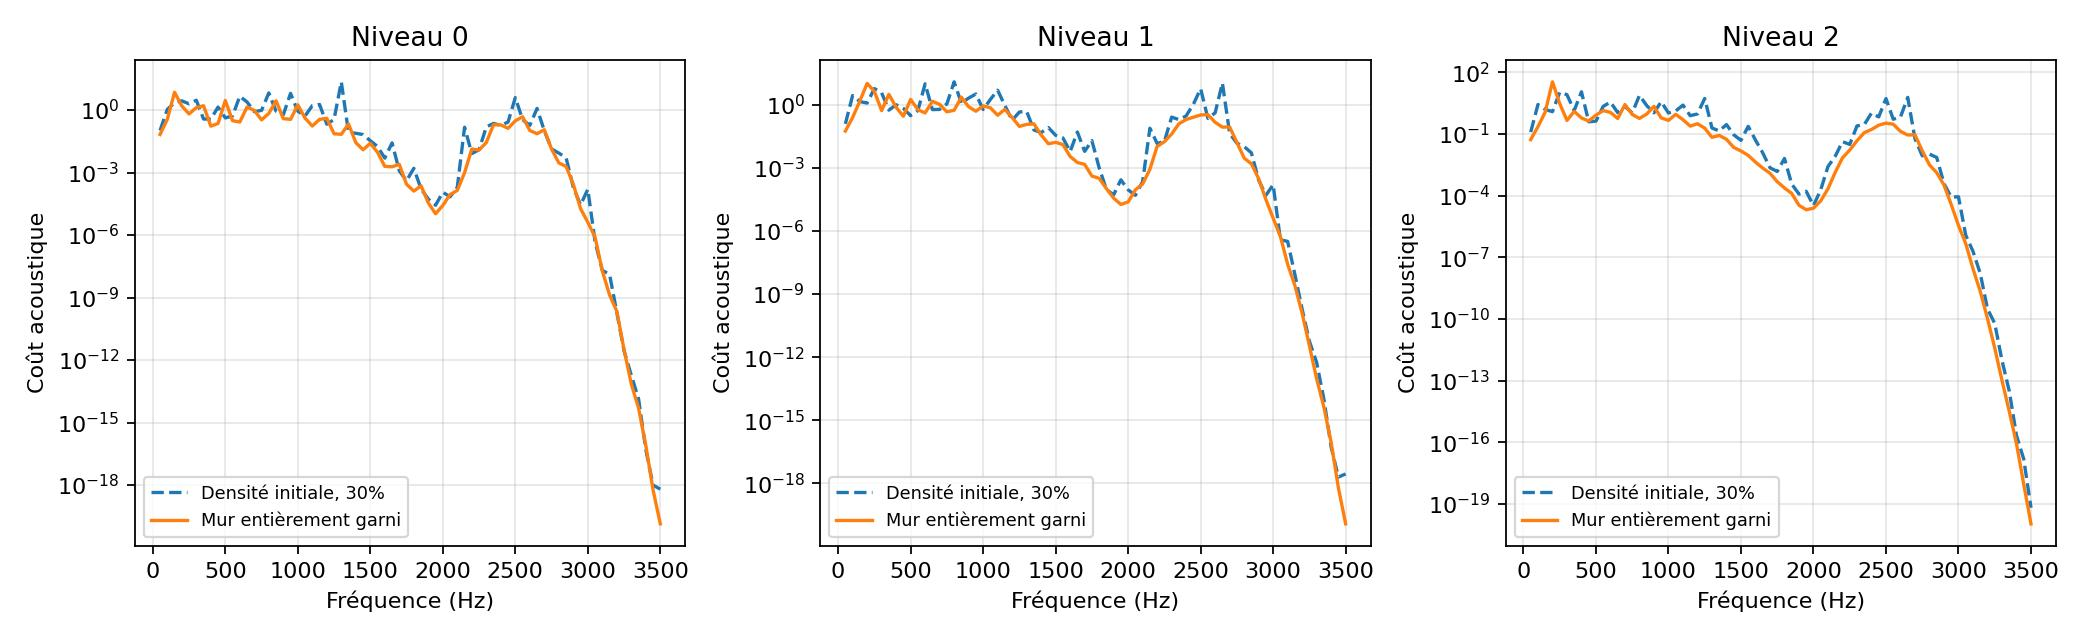
\includegraphics[width=1\textwidth,height=.50\textheight,keepaspectratio]{resultats_monofrequence/fig_repartition_partielle_et_complete.jpg}
\caption{Coûts des répartitions partielle et complète}
\end{figure}
{\small Densité initiale de moyenne 30\,\% ; référence entièrement garnie.}
\python{\code{project_density}, \code{evaluate_spectrum}}
\end{frame}

\begin{frame}[c]{Optimiser séparément des fréquences critiques}
\question{Diminution du coût à une fréquence choisie sur chaque mur.}
\begin{figure}
\centering
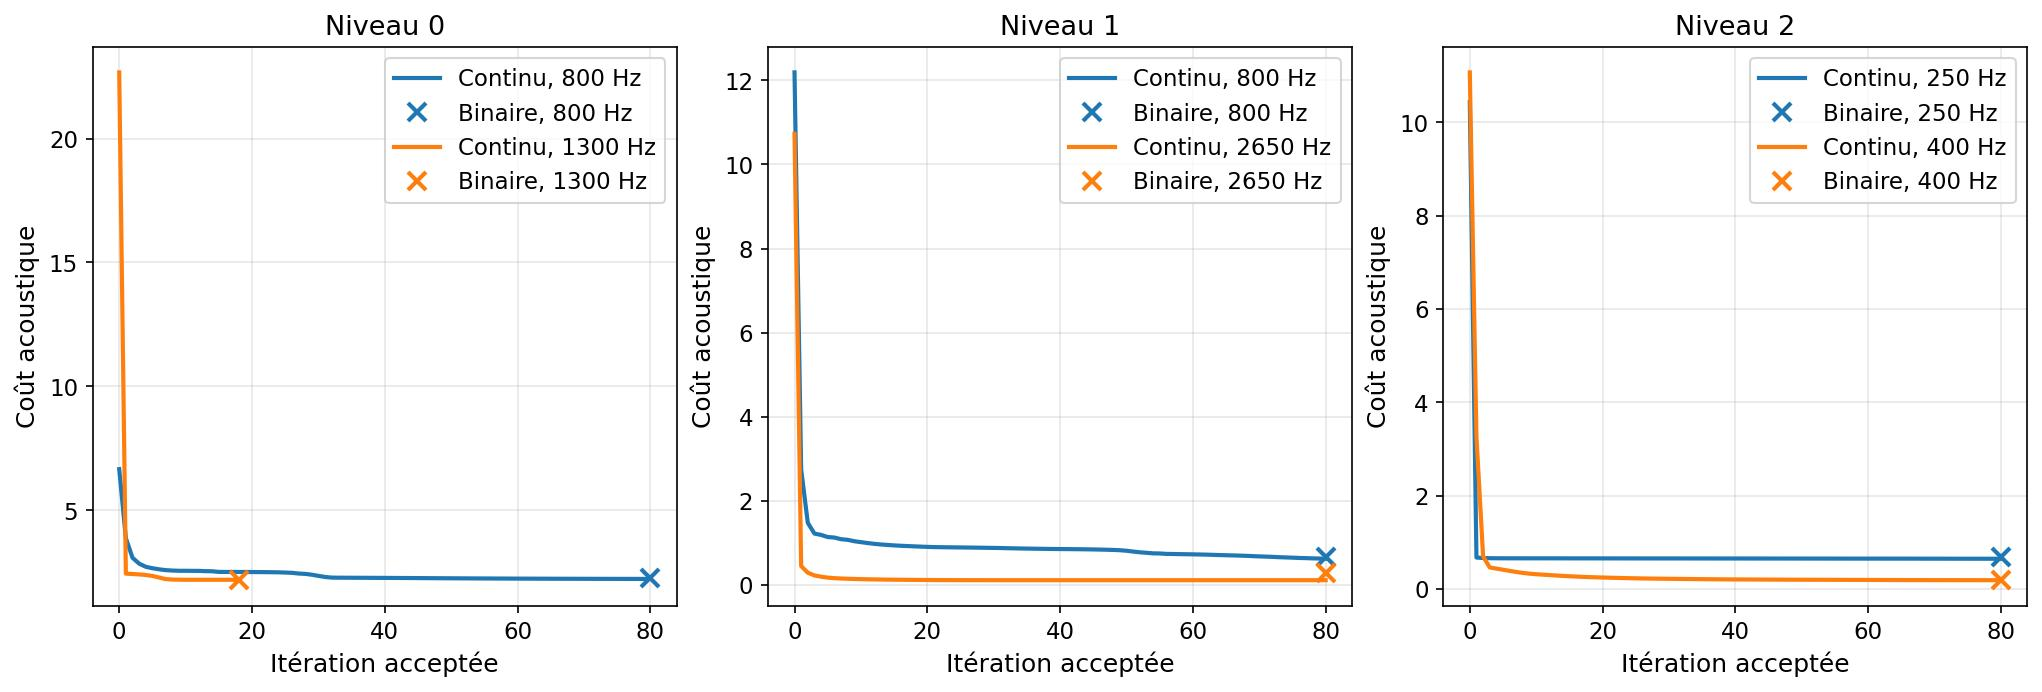
\includegraphics[width=1\textwidth,height=.55\textheight,keepaspectratio]{resultats_monofrequence/fig_historiques_monofrequence.jpg}
\caption{Historiques du coût aux fréquences critiques}
\end{figure}
{\small 80 itérations au maximum ; coûts continus et binaires évalués séparément.}
\python{\code{optimize_single_frequency}, \code{plot_single_frequency_details}}
\end{frame}

\begin{frame}[c]{Relier le placement au champ de pression}
\question{Comparaison des champs avant et après optimisation du placement.}
\begin{figure}
\centering
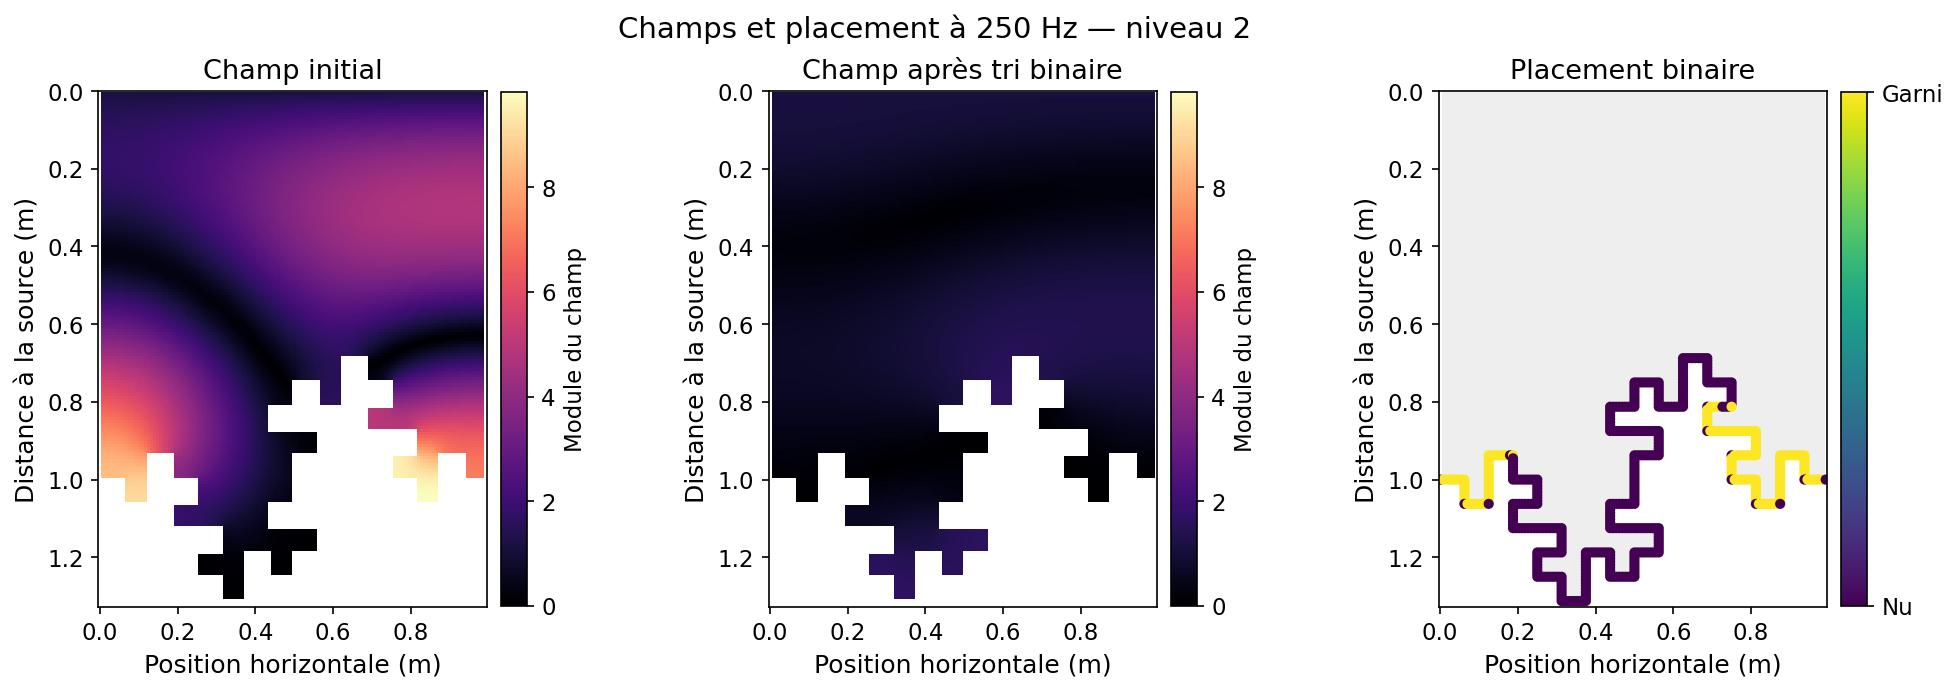
\includegraphics[width=1\textwidth,height=.55\textheight,keepaspectratio]{resultats_monofrequence/fig_champs_placement_monofrequence.jpg}
\caption{Champs initial et optimisé et placement binaire}
\end{figure}
{\small Même échelle de couleurs ; 154 points garnis après le passage binaire.}
\python{\code{binarize_chi}, \code{plot_single_frequency_details}}
\end{frame}

\section{Placement multifréquence}
\begin{frame}{Rappel du plan}
\footnotesize
\tableofcontents[currentsection,sectionstyle=show/shaded,subsectionstyle=show/shaded]
\end{frame}
\subsection{Réponse sur la bande}

\begin{frame}[c]{Réévaluer chaque placement sur toute la bande}
\question{Efficacité fréquentielle des placements optimisés à une seule fréquence.}
\begin{figure}
\centering
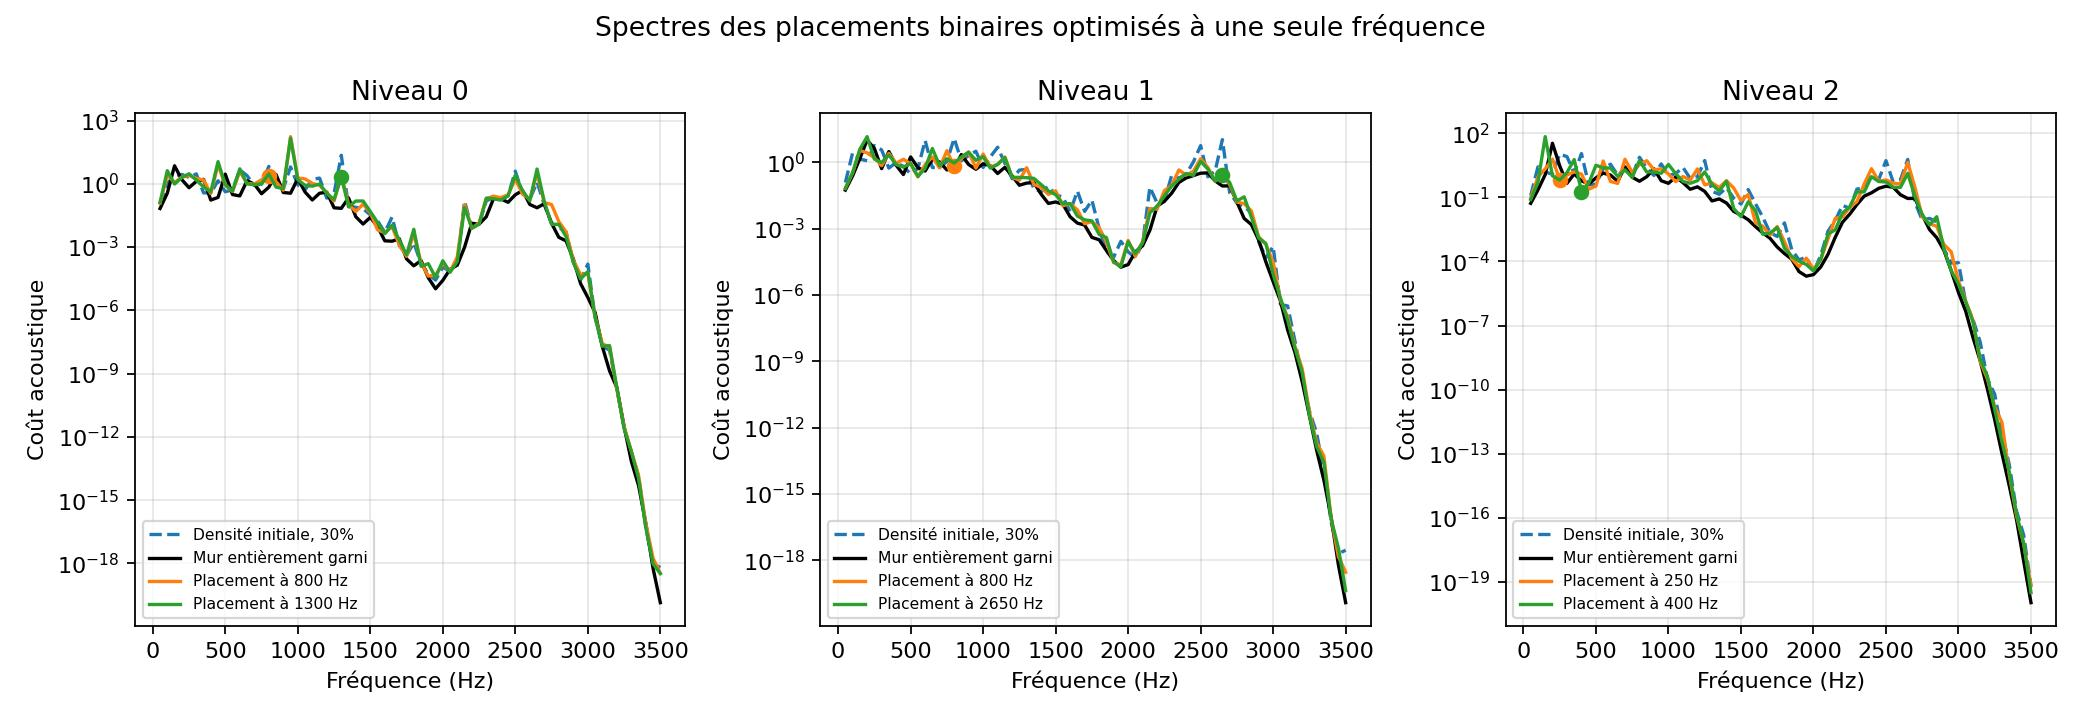
\includegraphics[width=1\textwidth,height=.50\textheight,keepaspectratio]{resultats_multifrequence/fig_spectres_placements_monofrequence.jpg}
\caption{Spectres des placements optimisés à une fréquence}
\end{figure}
{\small Chaque placement binaire est évalué sur la bande, au-delà de sa fréquence cible.}
\python{\code{evaluate_spectrum}}
\end{frame}

\begin{frame}[c]{Rechercher un placement commun à plusieurs fréquences}
\question{Formulation du critère multifréquence.}
On choisit trois fréquences critiques et on minimise leur coût moyen.
\begin{equation*}
J_{\mathcal F}(\chi)=\frac1{m}\sum_{r=1}^{m}J_{f_r}(\chi)
\qquad m=3
\end{equation*}
Le gradient est calculé à partir des mêmes fréquences.
\begin{equation*}
\nabla J_{\mathcal F}(\chi)=\frac1m\sum_{r=1}^{m}\nabla J_{f_r}(\chi)
\end{equation*}
\begin{itemize}
\item Une seule répartition $\chi$ pour tous les problèmes de Helmholtz.
\item L'amplitude de source est déjà dans le champ, donc dans le coût.
\end{itemize}
\python{\code{select_peak_indices}, \code{optimize_multi_frequency}}
\end{frame}

\begin{frame}[c]{Observer le coût moyen et les coûts individuels}
\question{Évolution du critère pendant l'optimisation multifréquence.}
\begin{figure}
\centering
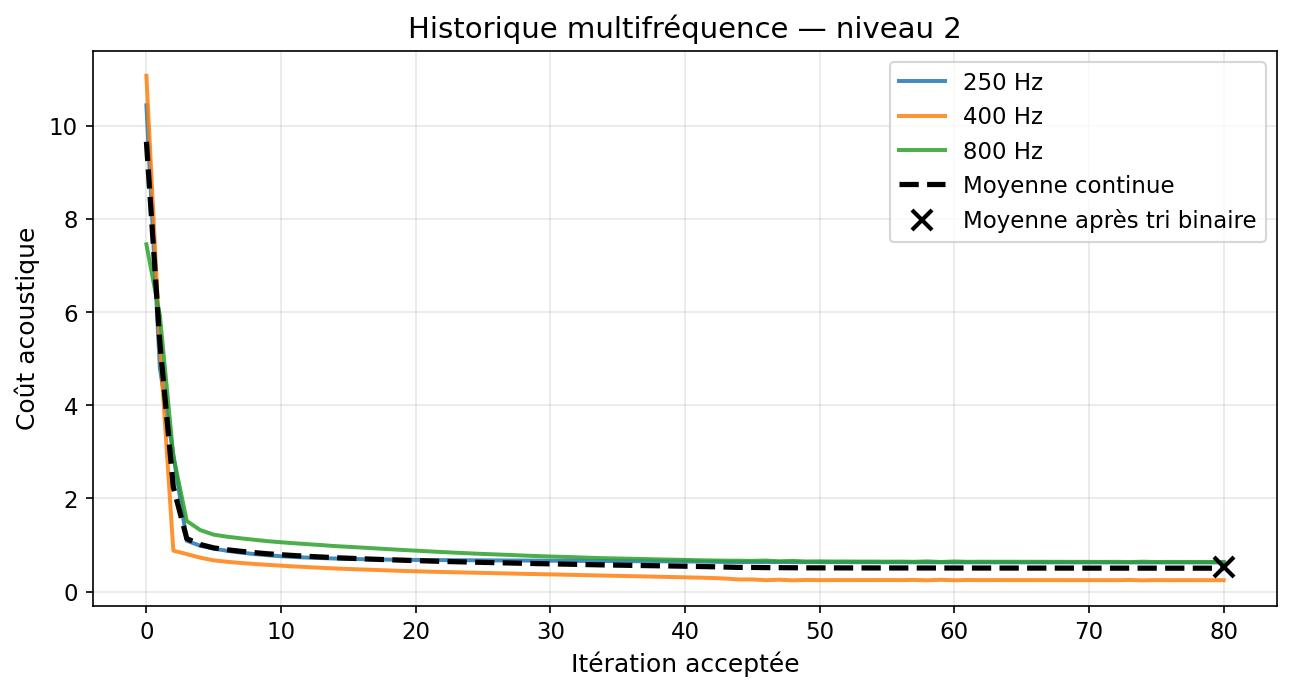
\includegraphics[width=1\textwidth,height=.55\textheight,keepaspectratio]{resultats_multifrequence/fig_historique_multifrequence.jpg}
\caption{Coût moyen et coûts des fréquences retenues pendant la descente}
\end{figure}
{\small La moyenne guide la descente ; chaque coût individuel est également tracé.}
\python{\code{optimize_multi_frequency}, \code{plot_multifrequency_details}}
\end{frame}

\begin{frame}[c]{Évaluer le placement multifréquence sur la bande}
\question{Comparaison avec les placements à une fréquence et la paroi entièrement garnie.}
\begin{figure}
\centering
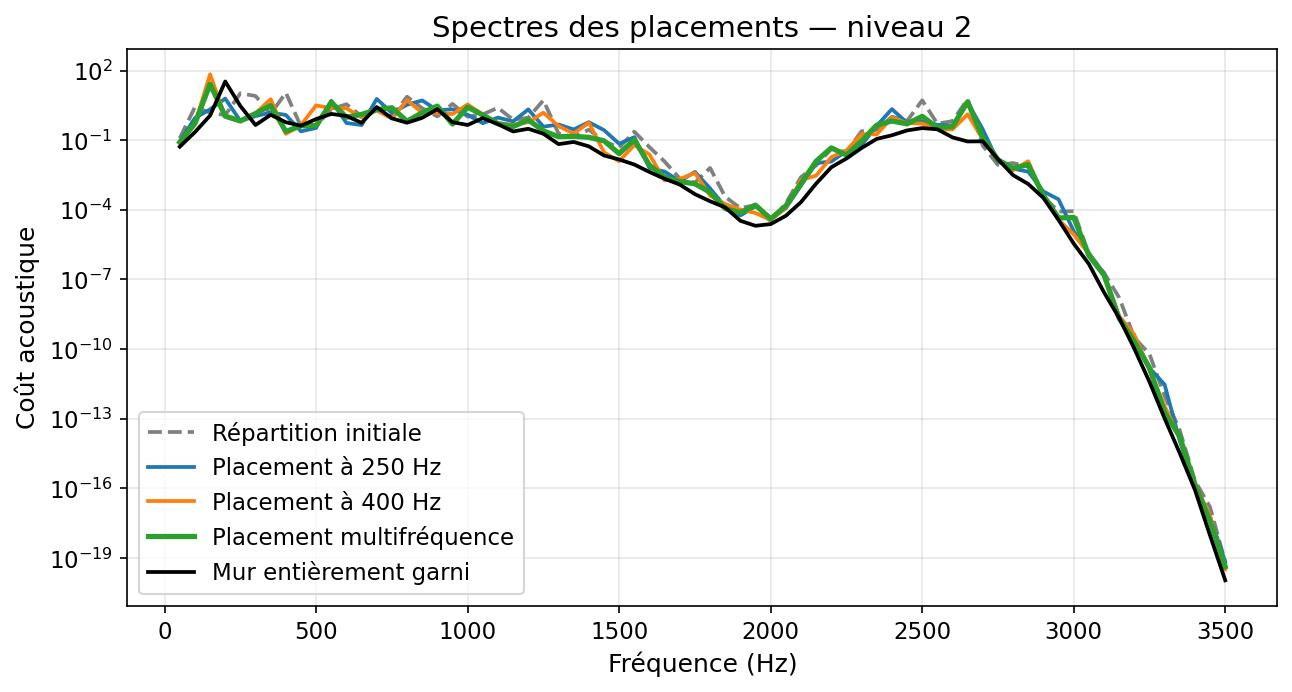
\includegraphics[width=1\textwidth,height=.55\textheight,keepaspectratio]{resultats_multifrequence/fig_spectre_multifrequence.jpg}
\caption{Spectres des répartitions initiale, monofréquences et multifréquence}
\end{figure}
{\small Les mêmes placements binaires sont conservés sur toute la bande étudiée.}
\python{\code{evaluate_spectrum}, \code{plot_multifrequency_details}}
\end{frame}

\subsection{Quantité de matériau}
\begin{frame}[c]{Rechercher la meilleure quantité parmi les fractions testées}
\question{Variation de la quantité d'absorbant à une ou plusieurs fréquences.}
\begin{figure}
\centering
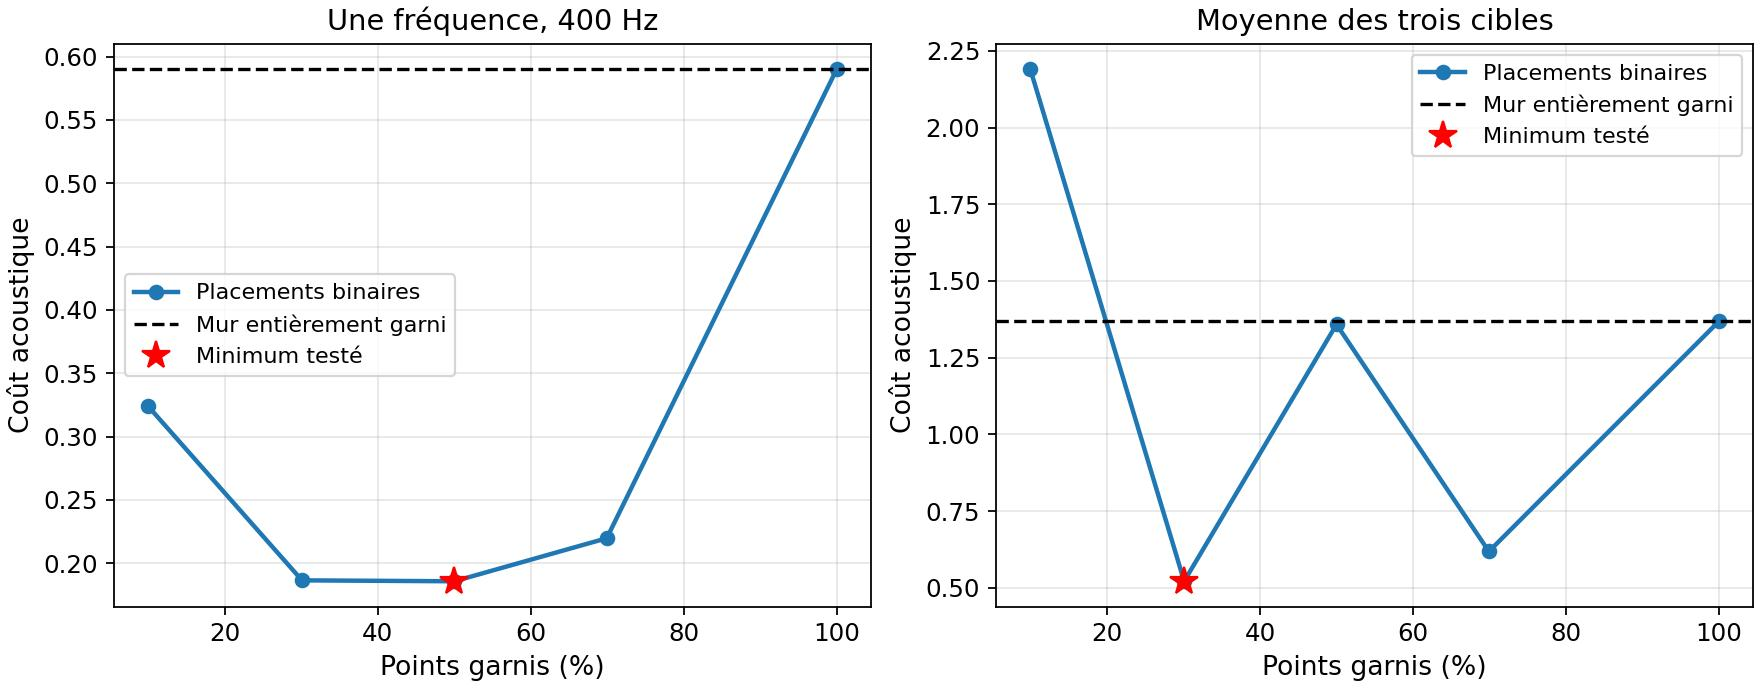
\includegraphics[width=1\textwidth,height=.55\textheight,keepaspectratio]{resultats_multifrequence/fig_quantite_niveau_deux.jpg}
\caption{Coût selon la fraction garnie au niveau 2}
\end{figure}
{\small Niveau 2 : à 400 Hz ou à trois fréquences ; fractions testées de 10 à 100\,\%.}
\python{\code{study_multifrequency_placement_and_coverage}, \code{plot_coverage_details}}
\end{frame}

\section{Comparaison des dispositifs}
\begin{frame}{Rappel du plan}
\footnotesize
\tableofcontents[currentsection,sectionstyle=show/shaded,subsectionstyle=show/shaded]
\end{frame}
\subsection{Répartition et excitation}

\begin{frame}[c]{Mesurer l'effet du passage au placement binaire}
\question{Performances des répartitions continue, binaire et mixte.}
\begin{figure}
\centering
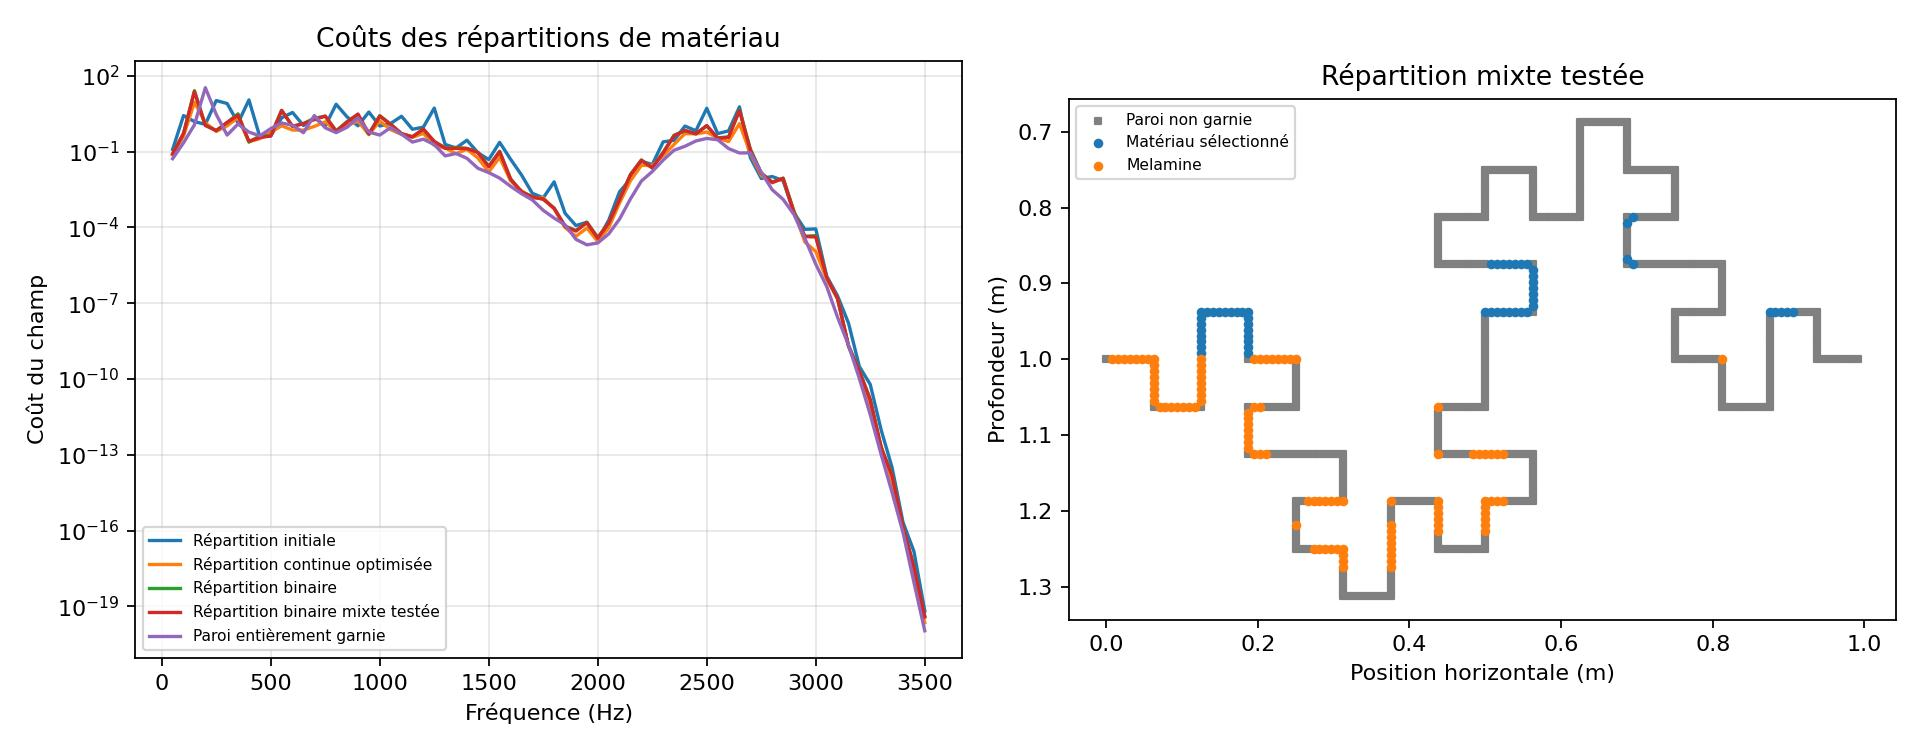
\includegraphics[width=1\textwidth,height=.50\textheight,keepaspectratio]{resultats_comparaison_dispositifs/fig_repartitions_binaire_et_mixte.jpg}
\caption{Spectres et carte d'une répartition à deux matériaux}
\end{figure}
{\small Coût recalculé après binarisation et après ajout du second matériau en partie basse.}
\python{\code{compare_absorber_configurations}}
\end{frame}

\begin{frame}[c]{Tester différents profils de source}
\question{Sensibilité du résultat au profil imposé sur le bord d'entrée.}
\begin{figure}
\centering
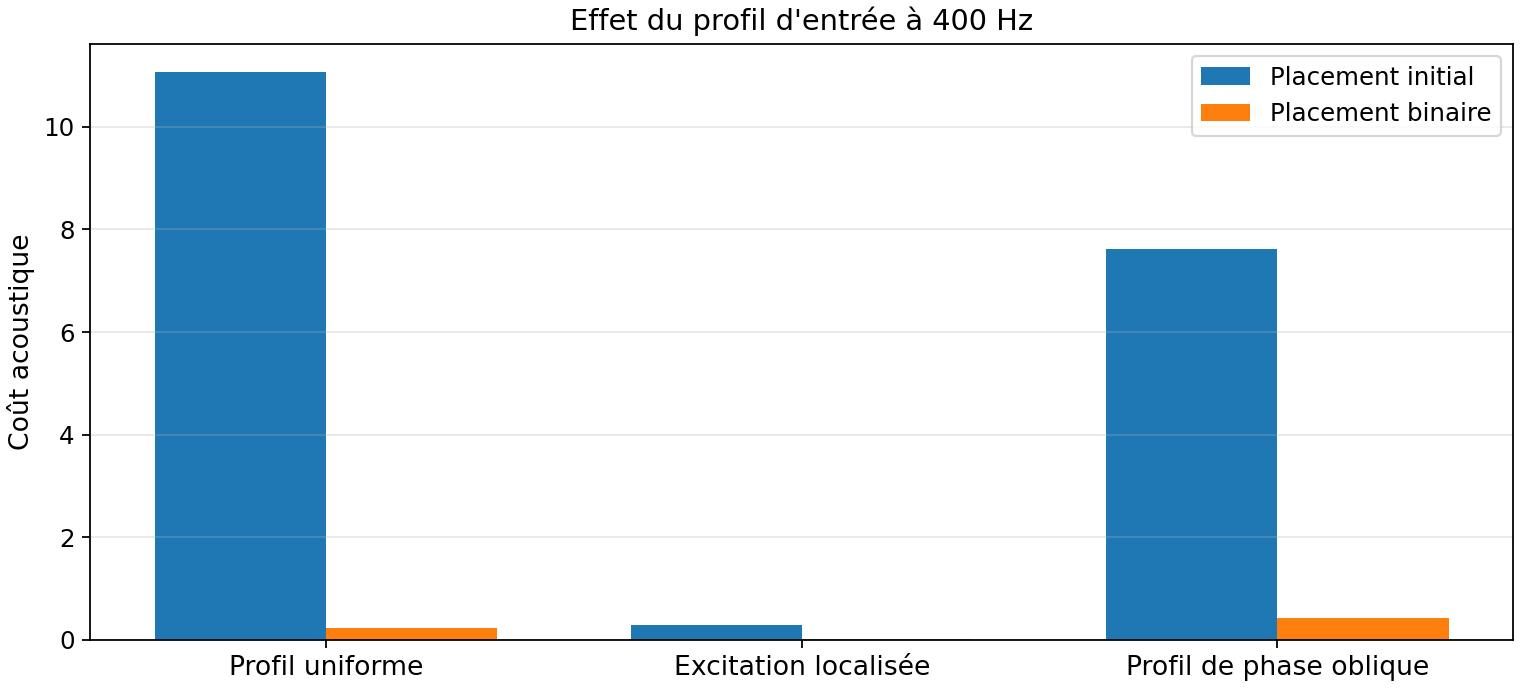
\includegraphics[width=1\textwidth,height=.55\textheight,keepaspectratio]{resultats_comparaison_dispositifs/fig_cout_profils_sources.jpg}
\caption{Coûts des profils uniforme, localisé et oblique}
\end{figure}
{\small Même somme d'amplitudes au carré sur le bord ; paroi et coefficient conservés.}
\python{\code{FastHelmholtzSolver.update_rhs}, \code{plot_source_profile_costs}}
\end{frame}

\subsection{Bilan et candidat}
\begin{frame}[c]{Comparer les matériaux et les niveaux géométriques}
\question{Choix d'un dispositif à partir des performances calculées.}
\begin{figure}
\centering
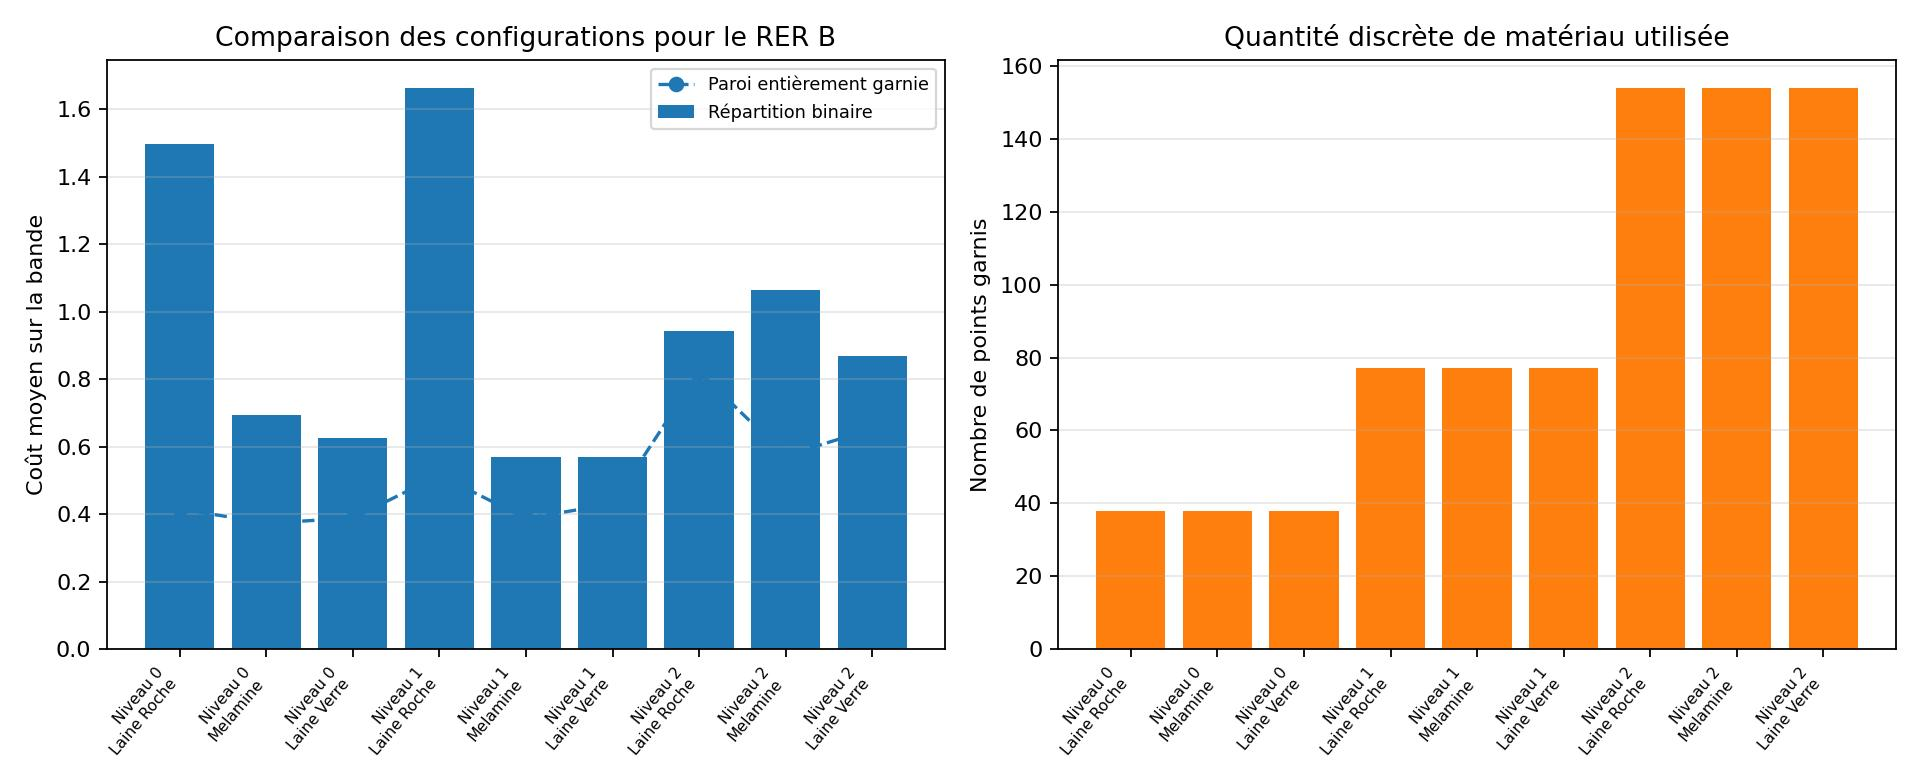
\includegraphics[width=1\textwidth,height=.50\textheight,keepaspectratio]{resultats_comparaison_dispositifs/fig_comparaison_dispositifs_resonics.jpg}
\caption{Coût moyen sur la bande et nombre de points garnis}
\end{figure}
{\small À 30\,\% : 38, 77 et 154 points garnis aux niveaux 0, 1 et 2.}
\python{\code{compare_absorber_configurations}, \code{mean_cost}}
\end{frame}

\begin{frame}[c]{Comparer les candidats avec le même budget discret}
\question{Comparaison des dispositifs à nombre de points garnis identique.}
\begin{figure}
\centering
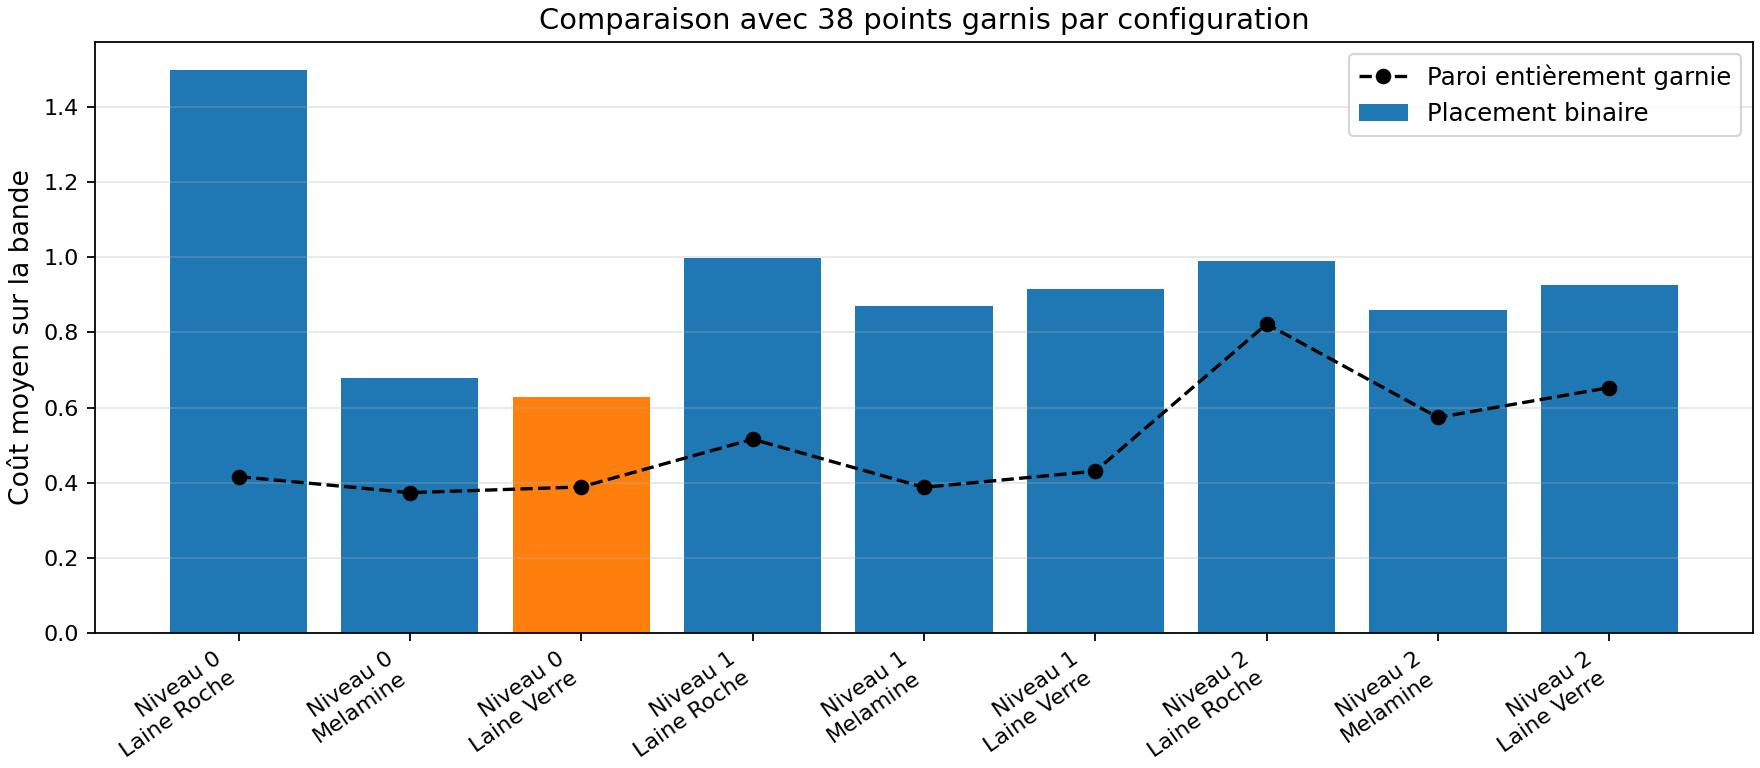
\includegraphics[width=1\textwidth,height=.50\textheight,keepaspectratio]{resultats_comparaison_dispositifs/fig_comparaison_budget_identique.jpg}
\caption{Coûts des configurations à budget discret identique}
\end{figure}
{\small Même budget final : 38 points ; meilleures répartitions binaires obtenues.}
\python{\code{compare_absorber_configurations}, \code{combine_comparable_configurations}}
\end{frame}

\begin{frame}[c]{Retenir un candidat dans le modèle étudié}
\question{Bilan du choix de matériau, de géométrie et de placement.}
À budget discret identique, le coût moyen le plus faible correspond à :
\begin{table}
\centering
\begin{tabular}{ll}
\toprule
Matériau & \RecommendedMaterial\\
Niveau du mur & \RecommendedLevel\\
Points garnis / points de Robin & \RecommendedCoveredNodes\,/\,\RecommendedRobinNodes\\
\bottomrule
\end{tabular}
\caption{Caractéristiques du candidat retenu}
\end{table}
Le coût moyen sur la bande est calculé par intégration fréquentielle.
\begin{equation*}
\overline J=\frac1{3500-50}\int_{50}^{3500}J_f\dd f
=\RecommendedBandCost
\end{equation*}
{\small La mélamine donne le plus faible maximum échantillonné : \BestMaximumValue.}
\end{frame}

\begin{frame}[c]{Mesurer l'intérêt du placement à quantité identique}
\question{Comparaison initiale, placement retenu et référence complète.}
\begin{figure}
\centering
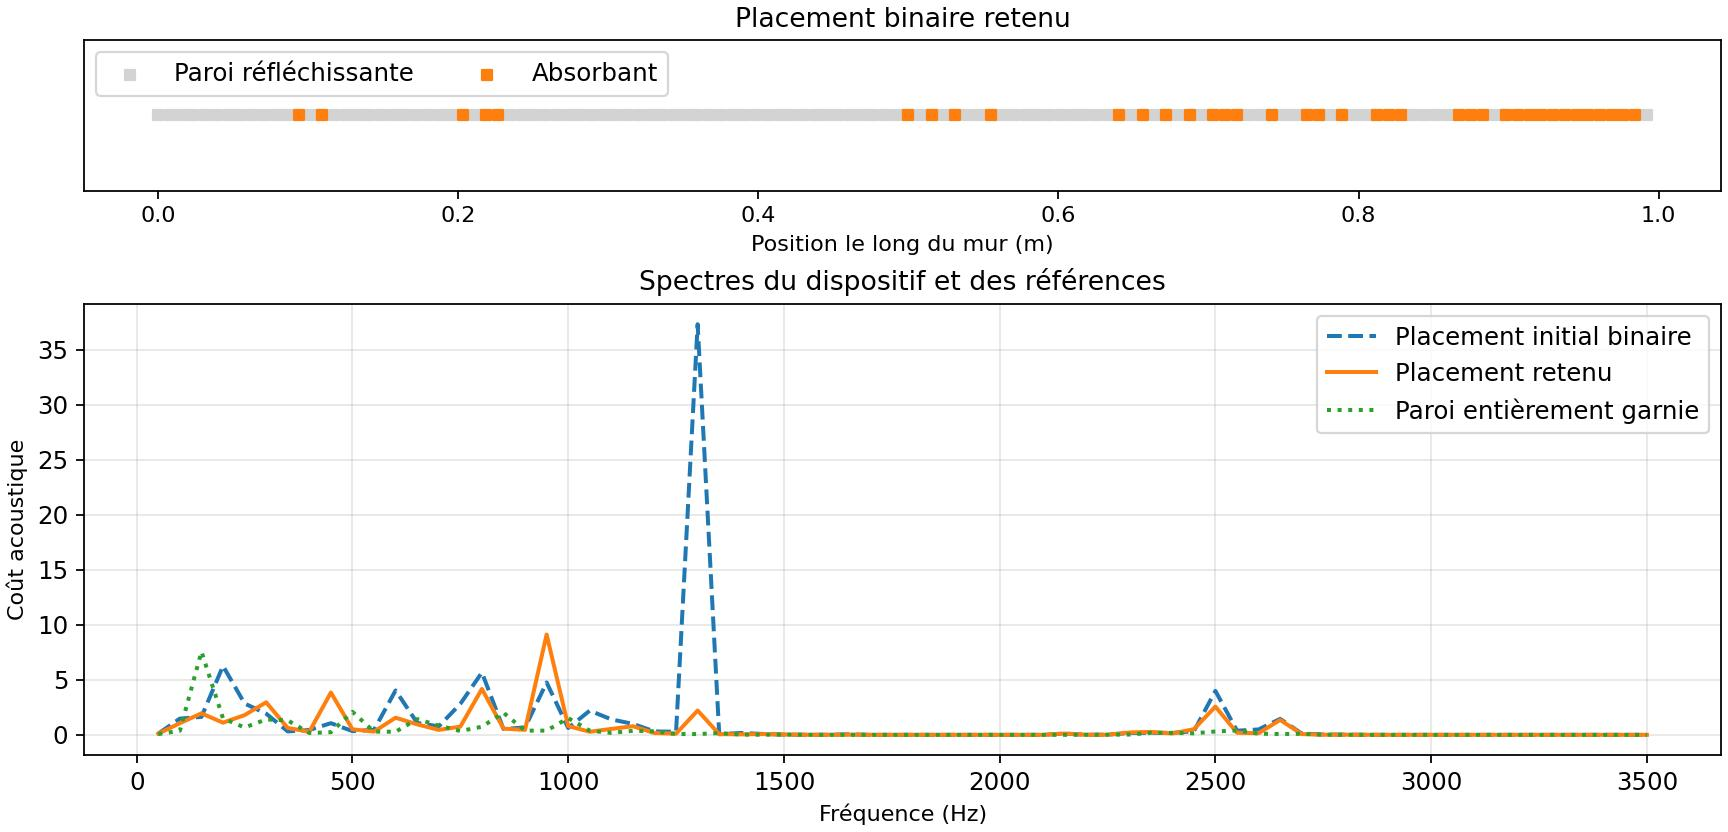
\includegraphics[width=1\textwidth,height=.50\textheight,keepaspectratio]{resultats_comparaison_dispositifs/fig_dispositif_retenu.jpg}
\caption{Placement et spectres du mur plan en laine de verre}
\end{figure}
{\small À 38 points garnis : coût moyen réduit de \SelectedBandReduction\,\% par rapport au placement initial binaire.}
\python{\code{evaluate_selected_configuration}, \code{plot_selected_configuration}}
\end{frame}

\begin{frame}[c]{Conclusion}
\begin{itemize}
\item \textbf{Matériau :} coefficient complexe identifié à chaque fréquence.
\item \textbf{Placement :} descente projetée, puis coût binaire recalculé.
\item \textbf{Comparaison :} spectres, fraction garnie et sensibilité à la source.
\end{itemize}
\medskip
\centering
\textbf{Un panneau se choisit par sa réponse sur la bande et sa quantité de matériau.}
\medskip
\begin{itemize}
\item Étape suivante : affiner les pics, les petites inclusions et la mesure de longueur garnie.
\end{itemize}
\end{frame}

\begin{frame}{Références}
\footnotesize
\begin{thebibliography}{9}
\bibitem{cours} A. Rozanova-Pierrat. \emph{Contrôle des Ondes}. Polycopié de cours, CentraleSupélec, 2026.
\bibitem{sncf} SNCF Réseau. \emph{Nos engagements pour la réduction du bruit ferroviaire}, 2026.
\bibitem{quierail} DELTABLOC. \emph{PHONOBLOC -- Série Special Rail}, documentation du fabricant.
\bibitem{felix} S. Félix et al. \emph{Enhanced wave absorption through irregular interfaces}. EPL, 85, 14003, 2009.
\bibitem{placement} F. Magoulès et al. \emph{Frequency Range of a Non-Lipschitz Parametric Optimization of a Noise Absorption}. SIAM J. Control Optim., 63, 1267--1285, 2025.
\end{thebibliography}
\end{frame}
\end{document}
